\chapter{Resultados}
\label{chap:analiseresultados}
Inicialmente para criação da arquitetura especificada na seção \ref{chap:arquitetura}, criou-se o serviço de \textit{Command}, o qual é a porta de entrada entre a interface de usuário e a arquitetura, este serviço tem a função de receber os dados da interface (dispositivo embarcado), validá-los e inserir na fila de mensagens, a qual foi montada se utilizando o Kafka, é através deste micro serviço que um carro terá a sua sessão criada (\textit{Command Session}), informará dados sobre a localização (\textit{Command Track}), ou ainda informações de alerta (\textit{Command Warning}), para isso, como pode ser observado no apêndice \ref{ap:sessioncommand}, se tem as validações de campos para cada um dos modelos de dados, no caso das informações referentes a sessão se tem informações sobre a marca, modelo, placa e  proprietário, no modelo de dados de localização se tem o identificador da sessão, nível de combustível, latitude, longitude e velocidade, e no modelo de dados referentes a alertas o identificador da sessão e o alerta emitido pelo veículo. Todos estes dados são manipulados e recebidos no formato \textit{JavaScript Object Notation} (JSON) por questões de velocidade e uso de memória. Ainda no apêndice  \ref{ap:sessioncommand} é apresentado todos os comandos de envio para a fila do Kafka de cada um dos modelos de dados.

Seguindo a arquitetura, se fez necessário a configuração da fila de mensagens (Kafka), a qual tem a função de armazenar uma informação por um determinado tempo até que ela expire depois de um tempo pré configurado. Para isso utilizou-se imagens Docker vindas de repositórios oficiais, sendo necessário um contêiner com a imagem do Kafka Zookeeper, o qual é o sistema responsável por gerenciar os \textit{brokers} do Kafka, e outro contêiner com a imagem do Kafka Broker, no qual se tem os \textit{brokers} propriamente dito, cada um funcionando em um contêiner separado.

O próximo passo que se tem dentro da arquitetura é a criação do micro serviço \textit{Worker}, o qual tem a finalidade de ler dados da fila de mensagens e armazená-las nos bancos de dados, para isso este micro serviço foi criado em Clojure, contendo a conexão com o Kafka, além das conexões com os bancos de dados MongoDB e Datomic, o apêndice \ref{ap:sessionworker} mostra a retirada de dados da fila de mensagens e gravação dos dados nas duas bases de dados, de acordo com o tipo de informação contida na mensagem.

Por fim foram configurados os bancos de dados, os quais armazenam os dados vindos dos serviços de \textit{Workers} e os mantém para consultas instantâneas no caso do MongoDB, ou consultas históricas no caso do Datomic. Para os dois bancos de dados utilizou-se de imagens Docker oficiais com a base de dados armazenadas no \textit{host}, para que os dados fiquem disponíveis para todas as réplicas, fazendo a função de \textit{pipeline} entre os contêineres, mesmo quando estes sejam replicados.

Tendo os dados armazenados, para o processo de leitura destes dados criou-se o micro serviço \textit{Command Query} também em Clojure, o qual tem a função de ler os dados inseridos no MongoDB, sem passar pela fila de mensagens, diretamente ele realiza a função de busca no banco de dados de acordo com a informação requisitada, retornando para o usuário que requisitou a informação que passará a ser exibida na interface do usuário.

Todos os micro serviços  utilizados dentro da arquitetura apresentam-se encapsulados dentro de contêineres, estes porém, possuem a base inicial vinda de uma imagem Docker oficial, no caso destes micro serviços utilizou-se a imagem Java com \textit{Java SE Runtime Environment} (JRE) em sua versão 8, sendo assim, as alterações e configurações para o ambiente desejado se fizeram através do Dockerfile, que ao ser construído gera uma nova imagem com as alterações nele contidos, e para criação do contêiner basta especificar que a imagem a ser usada será esta nova imagem.

Tendo as imagens criadas, para facilitar o processo de instalação de toda a arquitetura no servidor desejado criou-se o arquivo Docker Compose, através dele são especificados os contêineres que serão instanciados, bem como as portas e variáveis de ambiente para cada micro serviço, é função  dele manter o funcionamento dos contêineres e reiniciá-los em caso de falha, através dele também foi possível maior facilidade quando necessário parar ou reiniciar algum serviço. Como mostrado no apêndice \ref{ap:dockercompose}, são criados os contêineres para os micro serviços tendo conexões para os bancos de dados e a fila de mensagens, desta forma no servidor em que é instalado a arquitetura é possível observar o  \textit{cluster} de contêineres funcionando, como apresentado na figura \ref{fig:dockerps}.

\begin{figure}[!h]
\caption{\label{fig:dockerps} Cluster de Contêineres}
\begin{center}
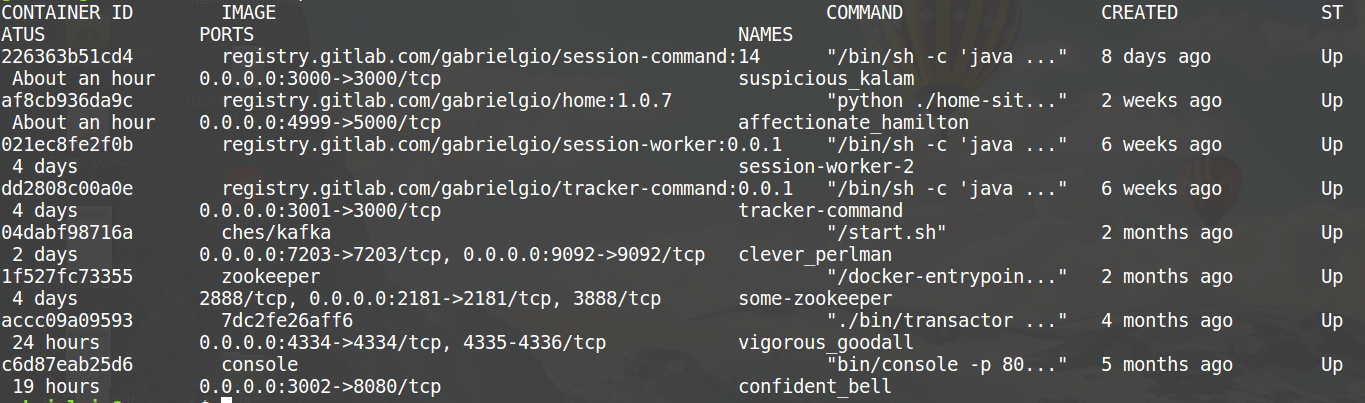
\includegraphics[scale=0.3]{dockerps}
\end{center}
%\legend{Fonte: \citeauthor{cqrs}, \citeyear{cqrs}} 
\end{figure}

Para verificação do fluxo de dados e validação da arquitetura criada, desenvolveu-se uma aplicação em Python, a qual apresenta uma interface para visualização dos veículos conectados a infraestrutura em tempo real, além das informações enviadas através destas conexões, se utilizando de \textit{sockets} para isso, tal aplicação se tornou útil para verificação das simulações que serão descritas na seção \ref{sec:testessistema}, pois através desta foi possível a visualização dos dados simulados de forma simples, como pode ser visto na figura \ref{fig:prototipo}.

\begin{figure}[!h]
\caption{\label{fig:prototipo} Visualização dos clientes}
\begin{center}
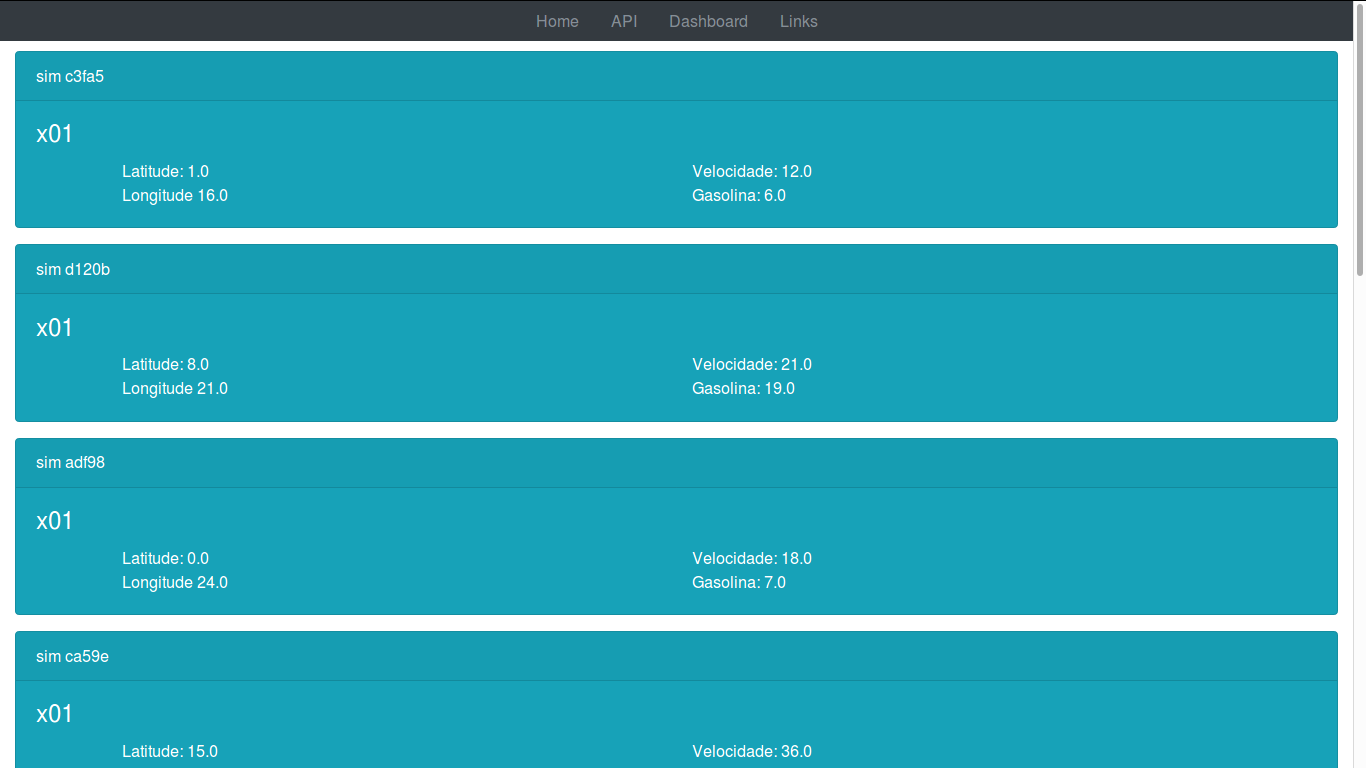
\includegraphics[scale=0.3]{prototipo}
\end{center}
%\legend{Fonte: \citeauthor{cqrs}, \citeyear{cqrs}} 
\end{figure}

\section{Testes de Sistema}
\label{sec:testessistema}
Para testes da arquitetura, realizou-se a instalação da mesma em um servidor no provedor de serviços \textit{Server as a Service} (SaaS) Azure, com uma máquina de 8 GB de memória e 2 núcleos de CPU, então para testes de carga na arquitetura, bem como teste de integridade de dados mesmo sobre alta pressão, foi desenvolvido um \textit{Mockup}, cujo o conceito é simular funcionalidades do sistema para que estas possam ser testadas de forma independente, sendo assim, dentro desta arquitetura os objetos \textit{mock} foram os carros e unidades de emergência, os quais tiveram seu comportamento simulado via \textit{software}, a fim de validar o armazenamento e fluxo de dados na arquitetura.

O \textit{Mockup} realizou-se por meio de um micro serviço escrito em Clojure, apresentado no apêndice \ref{ap:mockveiculos}, o qual cria uma quantidade de conexões pré-estabelecidas com o micro serviço \textit{Session Command} e envia dados fictícios como a criação de uma sessão, localização e informações referentes a nível de combustível e alertas em cada conexão criada, destas informações, nível de combustível e campos texto na criação da sessão se fizeram de forma aleatória, já a latitude e longitude se fez de forma a apresentar rotas reais para que estes pudessem receber os alertas das unidades de emergência, como mostra no apêndice \ref{ap:mockveiculos}, sendo assim, foi possível analisar o fluxo de dados dentro da arquitetura e verificar a veracidade dos dados armazenados, além de seu volume, como mostra a figura \ref{fig:dadosmongo} com dados armazenados no MongoDB e a figura \ref{fig:dadosdatomic} com dados do Datomic.

\begin{figure}[!h]
\caption{\label{fig:dadosmongo} Dados armazenados no MongoDB}
\begin{center}
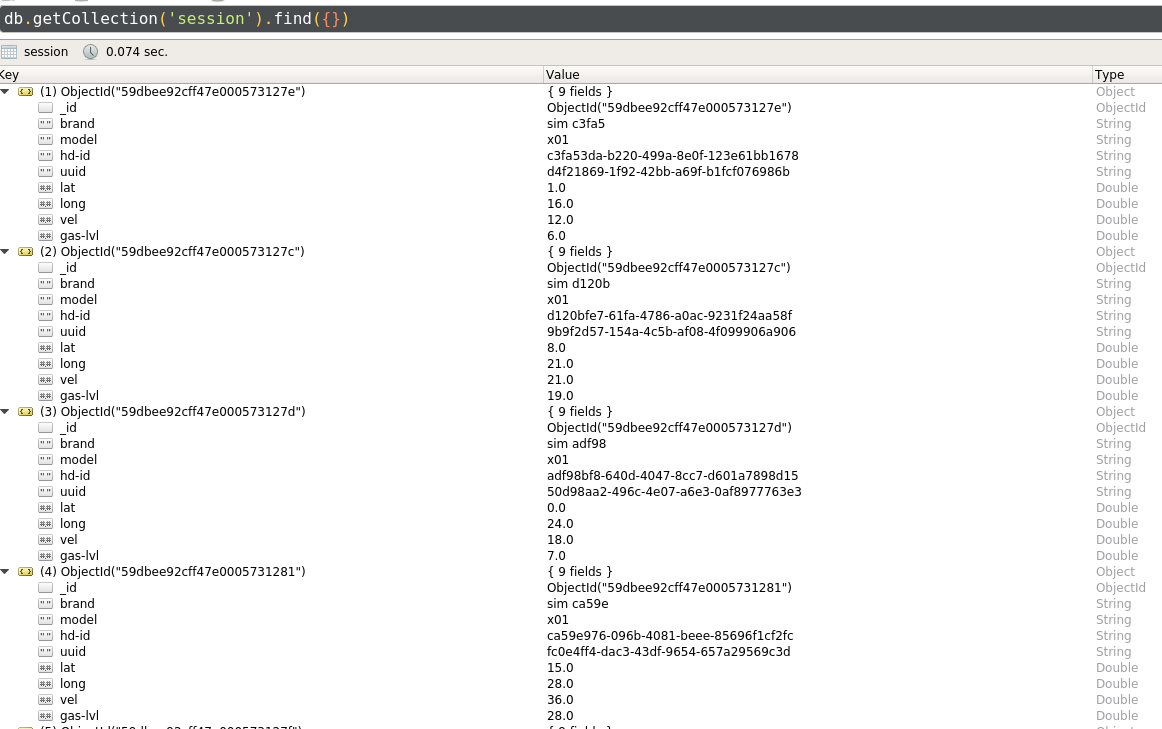
\includegraphics[scale=0.35]{dadosmongo2}
\end{center}
%\legend{Fonte: \citeauthor{cqrs}, \citeyear{cqrs}} 
\end{figure}

\begin{figure}[!h]
\caption{\label{fig:dadosdatomic} Dados armazenados no Datomic}
\begin{center}
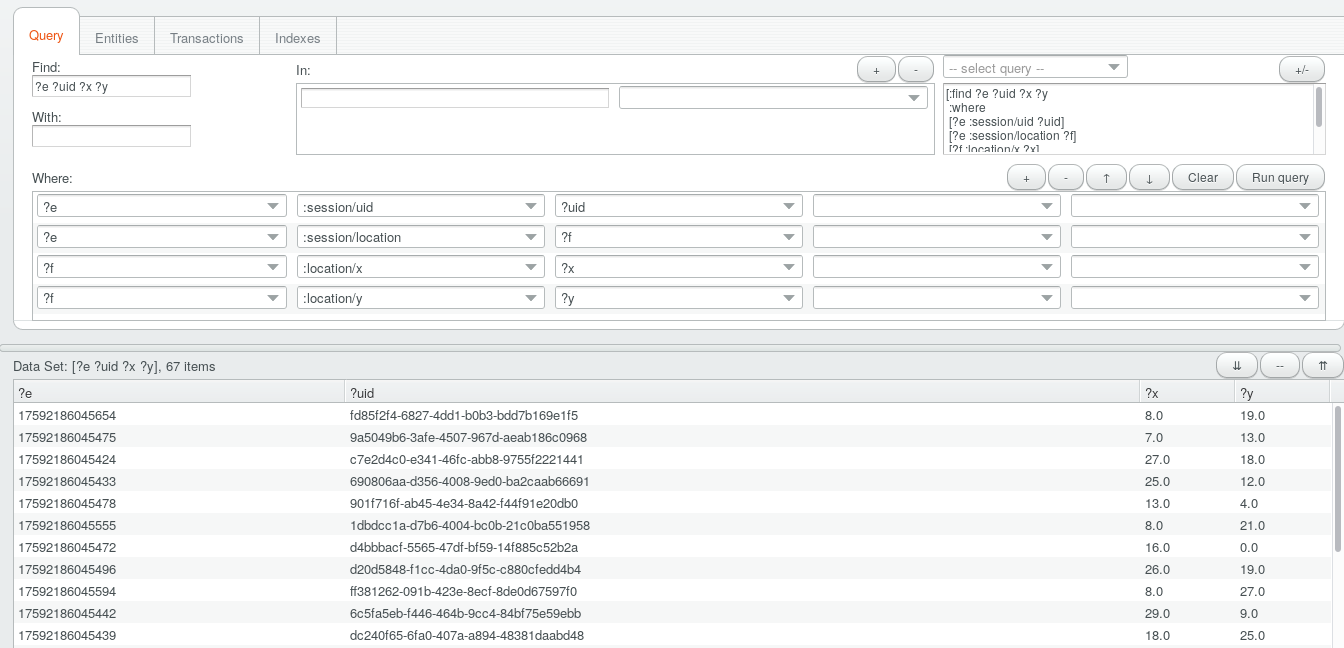
\includegraphics[scale=0.3]{dadosdatomic2}
\end{center}
%\legend{Fonte: \citeauthor{cqrs}, \citeyear{cqrs}} 
\end{figure}


Para testes de \textit{stress} se utilizou da ferramenta Locust, a qual teve a função de verificar a quantidade de usuários e conexões tal arquitetura suportaria, com os testes feitos se utilizando de uma máquina mestre e mais três escravas chegou-se aos resultados presentes na tabela \ref{tab:resultadoslocust}, em que é apresentado as quantidades de usuários, tempo de resposta, quantidade de requisições e requisições por segundo, se utilizando de até dois mil usuários, a cima disso o servidor líder e os escravos não suportavam simular mais usuários para gerar mais requisições na arquitetura, passando a falhar o servidor de testes e não a aplicação onde se encontra a arquitetura. Juntamente com a tabela a figura \ref{fig:graficoresultado} apresenta um gráfico com as requisições e tempo de respostas.

\begin{table}[h]
\centering
\caption{Resultados de teste de \textit{stress}}
\label{tab:resultadoslocust}
\begin{tabular}{ | l | l | l | l | l | l | }
\hline
	\textbf{Usuários} & \textbf{Requisições} & \textbf{Falhas} & \textbf{Respostas/s} & \textbf{Resposta(ms)} & \textbf{Requisições/s} \\ \hline
	50 & 1077 & 0 & 22 & 26 & 10.72 \\ \hline
	100 & 2133 & 0 & 20 & 21 & 21.55 \\ \hline
	150 & 2200 & 0 & 20 & 21 & 32.49 \\ \hline
	200 & 3831 & 0 & 22 & 27 & 43.29 \\ \hline
	250 & 5140 & 0 & 22 & 22 & 53.43 \\ \hline
	300 & 6636 & 0 & 22 & 26 & 65.12 \\ \hline
	350 & 6813 & 0 & 20 & 26 & 77.75 \\ \hline
	400 & 8188 & 0 & 21 & 27 & 89.04 \\ \hline
	450 & 8833 & 0 & 23 & 26 & 99.77 \\ \hline
	500 & 11173 & 0 & 21 & 25 & 111.33 \\ \hline
	550 & 13415 & 0 & 21 & 24 & 122.2 \\ \hline
	600 & 12980 & 0 & 22 & 26 & 134.18 \\ \hline
	650 & 14046 & 0 & 22 & 25 & 145.03 \\ \hline
	700 & 14451 & 0 & 22 & 26 & 155.15 \\ \hline
	750 & 15740 & 0 & 21 & 23 & 168.54 \\ \hline
	800 & 18473 & 0 & 22 & 23 & 178.27 \\ \hline
	850 & 16620 & 0 & 21 & 22 & 188.64 \\ \hline
	900 & 30161 & 0 & 21 & 23 & 199.67 \\ \hline
	950 & 13915 & 0 & 21 & 22 & 210.73 \\ \hline
	1000 & 13716 & 0 & 21 & 22 & 220.92 \\ \hline
	1100 & 20624 & 0 & 7 & 7 & 241.8 \\ \hline
	1200 & 14092 & 0 & 7 & 7 & 266.02 \\ \hline
	1300 & 5854 & 0 & 8 & 7 & 288.79 \\ \hline
	1400 & 18807 & 0 & 8 & 7 & 309.91 \\ \hline
	1500 & 15493 & 0 & 8 & 7 & 333.22 \\ \hline
	1600 & 10259 & 0 & 8 & 7 & 360.37 \\ \hline
	1700 & 20056 & 0 & 8 & 7 & 377 \\ \hline
	1800 & 15885 & 0 & 8 & 7 & 401.51 \\ \hline
	1900 & 21434 & 0 & 8 & 8 & 427.13 \\ \hline
	2000 & 15587 & 0 & 8 & 8 & 444.88 \\ \hline
\end{tabular}
\end{table}

\begin{figure}[!h]
\caption{\label{fig:graficoresultado} Gráfico de resultados do teste de \textit{stress}}
\begin{center}
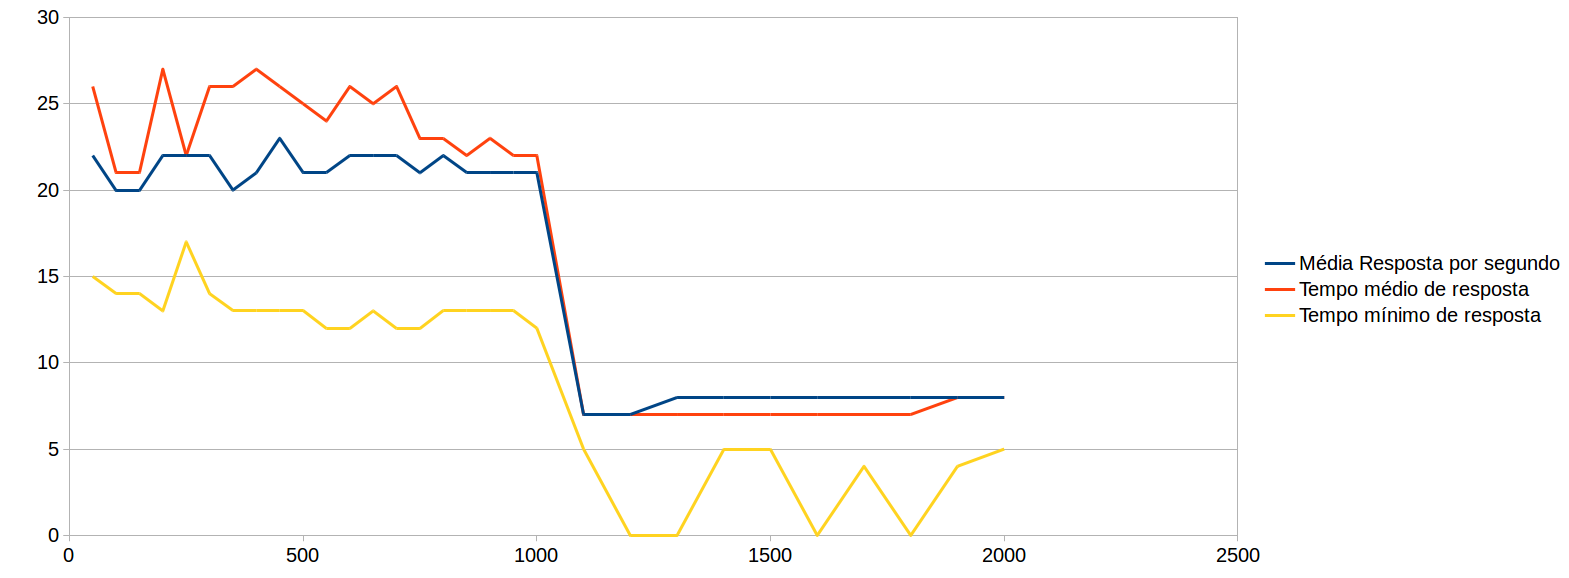
\includegraphics[scale=0.38]{graficoresultado}
\end{center}
%\legend{Fonte: \citeauthor{cqrs}, \citeyear{cqrs}} 
\end{figure}


\section{Discussão de Resultados}
\label{sec:discussãoresultados}
Através dos resultados apresentados é possível verificar que a arquitetura se adéqua ao propósito do seu desenvolvimento, apresentando uma alta escalabilidade e facilidade em sua implantação, através das ferramentas empregadas, quanto aos testes pode-se verificar que a arquitetura é válida quanto ao uso dela em uma análise de \textit{Big Data} se utilizado o banco de dados Datomic, e se prova ter rapidez quando trabalhado com os dados do MongoDB. 

A arquitetura se provou robusta mesmo quando funcionando em uma máquina de dois núcleos, possivelmente se utilizando de mais réplicas da fila de mensagens e do serviços de \textit{worker} em outros servidores,  os resultados seriam melhores, pois durante os testes o que mais sofria para o atendimento das requisições era os serviços de \textit{worker} que por gravarem dados no banco se tornam mais lentos.

No teste de \textit{stress} a arquitetura também se saiu bem, suportando uma pelo menos dois mil usuários conectados, que foi o número capaz de ser calculado pelos recursos que se possuíam para tal teste, sendo que esse número pode aumentar ao passo que se distribui mais a arquitetura em outros servidores, algo fácil de ser realizado, pois desde o início do trabalho o objetivo foi criar algo que se pudesse se escalar  facilmente.

Com relação ao seu desenvolvimento, ferramentas como Docker e Docker Compose provaram ser muito úteis quando o assunto é realizar \textit{deploy} de uma aplicação de forma rápida, diminuindo consideravelmente o tempo para instalação de todo o ambiente de produção, atingindo o objetivo de se ter uma arquitetura que fosse construída de forma ágil.

Visto os resultados de desempenho do servidor, é possível dizer que a arquitetura desenvolvida se enquadra em uma arquitetura de \textit{Big Data}, pois possui a velocidade na obtenção de resultados, sendo capaz de se analisar dados praticamente em tempo real, quanto a veracidade dos dados, a escolha do banco Datomic garantiu isso de forma a não perder registros muito menos causar alterações indesejadas neles, além de manter uma base histórica dos dados armazenados, mesmo quando a base de dados passou a crescer gerando um grande volume. 

Através do uso dos micro serviços notou-se também que a integração da arquitetura com qualquer outro dispositivo de IoT pode ser feita de forma fácil, pois nos próprios testes se teve um microsserviço em Clojure se conectando a infraestrutura e uma ferramenta de teste de \textit{stress} escrita em Python, desta forma independente da tecnologia utilizada nas pontas, ela se adaptaria facilmente à arquitetura independente da tecnologia empregada no IoT. 